\documentclass[tikz,margin=1mm]{standalone}


\begin{document}
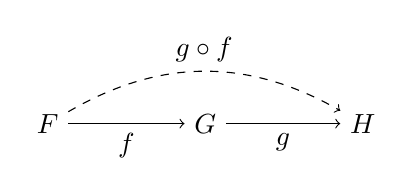
\begin{tikzpicture}[node distance=2cm, auto]
  \node (F) {$F$};
  \node[right of=F] (G) {$G$};
  \node[right of=G] (H) {$H$};

  \draw[->] (F) to node[swap] {$f$} (G);
  \draw[->] (G) to node[swap] {$g$} (H);

  \draw[->, dashed, bend left] (F) to node {$g \circ f$} (H); 
\end{tikzpicture}
\end{document}